\documentclass[12pt,a4paper]{article}

\usepackage{epcc}
%\usepackage{graphics}
\usepackage{graphicx}
\usepackage{pgfgantt}
\usepackage{array}

% This example file shows how a thesis can be laid out using Latex. It
% does not use any special local features so should be portable to other
% places.
%
% To produce myfile.pdf from myfile.tex type:
% 
% pdflatex myfile
%
% Note that pdflatex expects all included figures to be in PDF too. See
% the includegraphics command below.


% This document contains many cross-references and forward references,
% eg in constructing a table of contents, so Latex may need to be run
% twice to get all the references correct. If you need to run Latex twice
% you may get the warning:
% 
% LaTeX Warning: Label(s) may have changed. Rerun to get cross-references right


\begin{document}

\title{Software Development\\UI and Evaluation Plan}
\author{B098688 - s1671778}
\date{\today}

\makeEPCCtitle

\thispagestyle{empty}

\newpage

\pagenumbering{roman}

\tableofcontents


\newpage
\pagenumbering{arabic}

\section{Introduction}

This report will 

This report will provide a series of guidelines on how to proceed with the creation of a web application. The web application's code has been initiated by an unknown party, that is written in \texttt{html}, \texttt{JavaScript}, \texttt{python} and uses the web framework \texttt{flask}. Said code must be enhanced such that it fulfills the base requirements for the project. The skeleton of the web application has a few elements already built in. It is, however, very rough and needs much work to become a feasible end product. 

The first part of the report will briefly outline what is the intended project, and the background needed to understand what it is attempting to achieve. While this is being discussed, some of the important factors to keep in mind are highlighted. After this is done, several comments regarding issues in the provided code are made. Afterwards, solutions for most of these are proposed, and eventually presented in a \textit{time/effort} estimation plan. Finally, once the project has been understood, and its purpose is clear, risk analysis and management strategy are posed. For the latter, a Gantt chart is put together to act as a guide for the next steps: \textit{UI and Evaluation Plan} and \textit{Refactoring and Reflection}.

The management strategy in this small project will help make a successful end product. There are many factors to be analysed in order to properly develop the software development planning. Considering personal inexperience in web security, \texttt{flask}, \texttt{html}, and \texttt{JavaScript}, it is safe to assume that many issues with the program will be overlooked at the beginning. This means that the problems mentioned in this document will be a fraction of those that will actually be fixed in the later stages of the project. This will require allocating time to research on the aforementioned topics as well as choosing carefully the best development model. After careful consideration and taking into account that this project will need to cycle from the current code to an improved version a few times, the \textit{Waterfall with Subprojects} development model is going to be used.

Having mentioned how the lack of experience will impact the development model required, it is important to analyze how it will modify other elements of the project's progress. The best way to do this is most likely through the Gantt chart. In it, tasks that have to be completed and are related to areas of inexperience will need some time allocation for 'research' or 'practice', but this will decrease as more tasks of the same area are performed, i.e. account for knowledge growth. 

\section{Project Specifications}
\label{sec:concept}

The goal is to further develop a web based application that allows the user to generate a squad (Warband) for a tabletop game - with certain constraints. The application must allow users to create and edit squads with an unchangeable name, no more than 10 members, and no fewer than 1. The user begins with a Captain, that can become better with time, and has a limited amount of money to hire other regular team members, that cannot improve with time, and a special member, the Ensign, who, like the Captain, can evolve in time.

The idea of the web application is to check that all constraints are fulfilled for a user's Warband, and that if one or more are violated, a warning message is displayed such that the user is able to modify their decision. The base stats for each team member are shown in the Annex.

\subsection{New Warband}

A new Warband begins with \textbf{one} Captain and \textbf{500} credits. For a new Warband to be created, the following conditions must be met:

\begin{enumerate}
 \item Warband Name.
 \item Player Name.
 \item Positive number of credits.
 \item Captain: \begin{enumerate}
                 \item \textbf{ONE} per Warband.
                 \item Starts with \textbf{one} EXPERIENCE.
                 \item Must be assigned \textbf{one} SPECIALISM (Engineering, Psychology, Marksman, Tactics, Melee, Defence).
                 \item \textbf{One} Associated Skill must be assigned to the specified SPECIALISM: \begin{enumerate}
							  \item Engineering: [Repair, Sabotage, Augment].
							  \item Psychology: [Bolster, Terror, Counter].
							  \item Marksman: [Aim, Pierce, Reload].
							  \item Tactics: [Squad, Ambush, Surround].
							  \item Melee: [Block, Riposte, Dual].
							  \item Defence: [Shield, Sacrifice, Resolute].
							 \end{enumerate}
				 \item Must be given \textbf{one} WEAPONS/EQUIPMENT: \begin{enumerate}
				                                         \item Blaster: \textbf{5} credits.
				                                         \item Needle Gun: \textbf{12} credits.
				                                         \item Blade: \textbf{3} credits.
				                                         \item Cannon: \textbf{15} credits.
				                                         \item Whip: \textbf{5} credits.
				                                        \end{enumerate}
                \end{enumerate}
 \item Ensign: \begin{enumerate}
                \item Price of hiring: \textbf{250} credits.
                \item Maximum \textbf{ONE} (Warbands can be created without an Ensign).
                \item Must be assigned \textbf{one} SPECIALISM.
                \item Must be assigned \textbf{one} Associated Skill.
                \item Must be given \textbf{one} WEAPONS/EQUIPMENT.
               \end{enumerate}
 \item The total number of members is \textbf{10} (including the Captain and Ensign).
 \item Prices of hiring are: \begin{enumerate}
                              \item Augment Gorilla: \textbf{20} credits.
                              \item Lackey: \textbf{20} credits.
                              \item Security: \textbf{80} credits.
                              \item Engineer: \textbf{60} credits.
                              \item Medic: \textbf{50} credits.
                              \item Commando: \textbf{100} credits.
                              \item Combat Droid: \textbf{150} credits.
                             \end{enumerate}
\end{enumerate}

\subsection{Edit Warband}

When editing a Warband there is also a set of conditions that have to be met. They are outlined here.

\begin{enumerate}
 \item Can hire squad members as long as the total number of squad members does not exceed \textbf{10}, and as long as the Warband's number of credits does not become negative.
 \item Captain and Ensign can gain EXPERIENCE.
 \item Acquired EXPERIENCE can be traded for upgrades for Captain and Ensign (\textbf{10} EXPERIENCE points can be turned into \textbf{1} point for a Stat up to specified maximum values shown in the Appendix section).
 \item Can remove squad members, but their hiring price is \textbf{not} returned to the number of credits.
 \item The Captain can have up to \textbf{two} weapons and \textbf{four} items.
 \item The Ensign can have up to \textbf{one} weapon and \textbf{3} items.
 \item Weapons cost credits. Changing or adding weapons \textbf{cannot} result in a negative number of credits.
\end{enumerate}


\section{Identified Problems}

Now that the constraints of the teams have been covered, it is possible to go through the code to check missing or wrong information. But first, going through the current web application to see errors in its functioning is important. The following is a list of problems that are observed by working though the web application alone. 

\subsection{New Warband}

\begin{enumerate}
 \item The most obvious deficiency is the fact that Warbands are not linked to a specific player. This means that anyone can edit any Warband. The game must support more than one player, where only the team's owner can edit it, but all other players can see it.
 \item There is no way to go from the ``New Warband'' or ``Edit Warband'' pages to the ``Home'' page without using browser back button or address bar.
 \item There has been no attempt at testing the current product. For example, when attempting to generate an illegal ``New Warband'' (Captain without weapon / skill / specialism), an error message is given, but no explanation or way to return and fix the mistakes are provided.\\
 \begin{minipage}[t]{\linewidth}
 \centering
 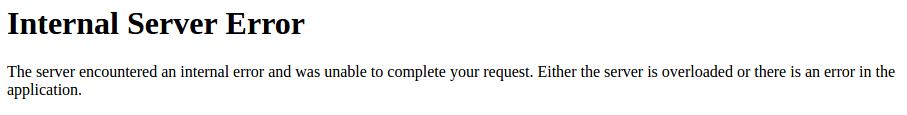
\includegraphics[width=1\textwidth]{img/warband_error}
 Generic error message.
 \end{minipage}
 
 \item The price of weapons is not discounted from the number of credits from the screen when creating a ``New Warband''.
 \item Neither Captain nor Ensign have ''Notes`` section, and merged ''Weapons and Equipment``, whereas the two should be different.
 \item The Ensign is called ``Apprentice'' for some reason - this is confusing.
 \item The cost of the ``Apprentice'' is 200 credits instead of 250 as it should. This and the previous item are actually related, and comprise a larger problem - the information from each team member is actually stored in the \texttt{python} code and separately in the \texttt{html/JavaScript} code. Due to this, the price on screen is 200 credits, but it actually subtracts 250 credits (as it should). 
 \item A 10 row table allows the player to fill out the form with up to 12 members (returns the generic error message when done so).\\
 \begin{minipage}[t]{\linewidth}
 \centering
 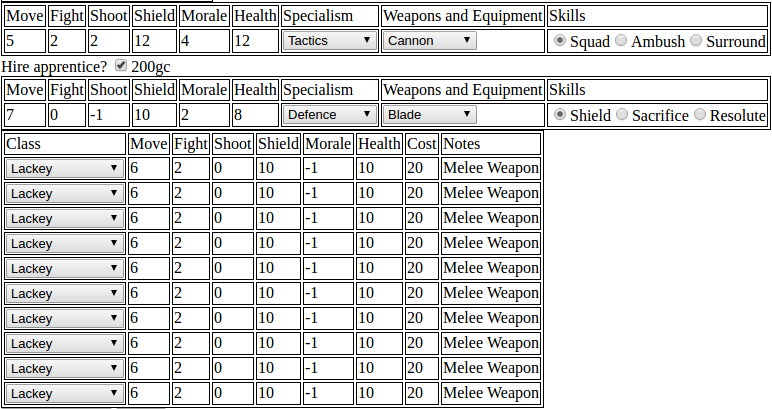
\includegraphics[width=1\textwidth]{img/twelve_members}
 Chance to include 12 members.
 \end{minipage}
 
 \item There is no method for handling attempts at creating a new Warband with a name that already exists. This has to be carefully thought out when including multiplayer - no two teams can have the same name, even if they are built by different players - involving the client is important for this decision.
 \item Consecutively creating new Warbands will accumulate the price of weapons and squad members (big problem).
 \item Trying to create two new Warbands without leaving the ``New Warband'' menu does not allow to select weapon for Captain.
 \item After creating a Warband with the Captain's weapon being a cannon, the next new Warband's Captain will also have a cannon, regardless of the choice of weapon.

\end{enumerate}

\subsection{Edit Warband}

\begin{enumerate}
 \item The most serious problem in the ``Edit Warband'' menu is the handling of credits. When editing the Warband the number of credits is modified erroneously:\\
 A new Warband with only a Captain with a cannon (15 credits) is generated. Then, in the ``Edit Warband'' page, clicking ``Create Warband'' decreases the number of credits by 15 (shown in the figures below). Like this, there are other errors with the credit handling in the ``Edit Warband'' page.\\
 \begin{minipage}[t]{\linewidth}
 \centering
 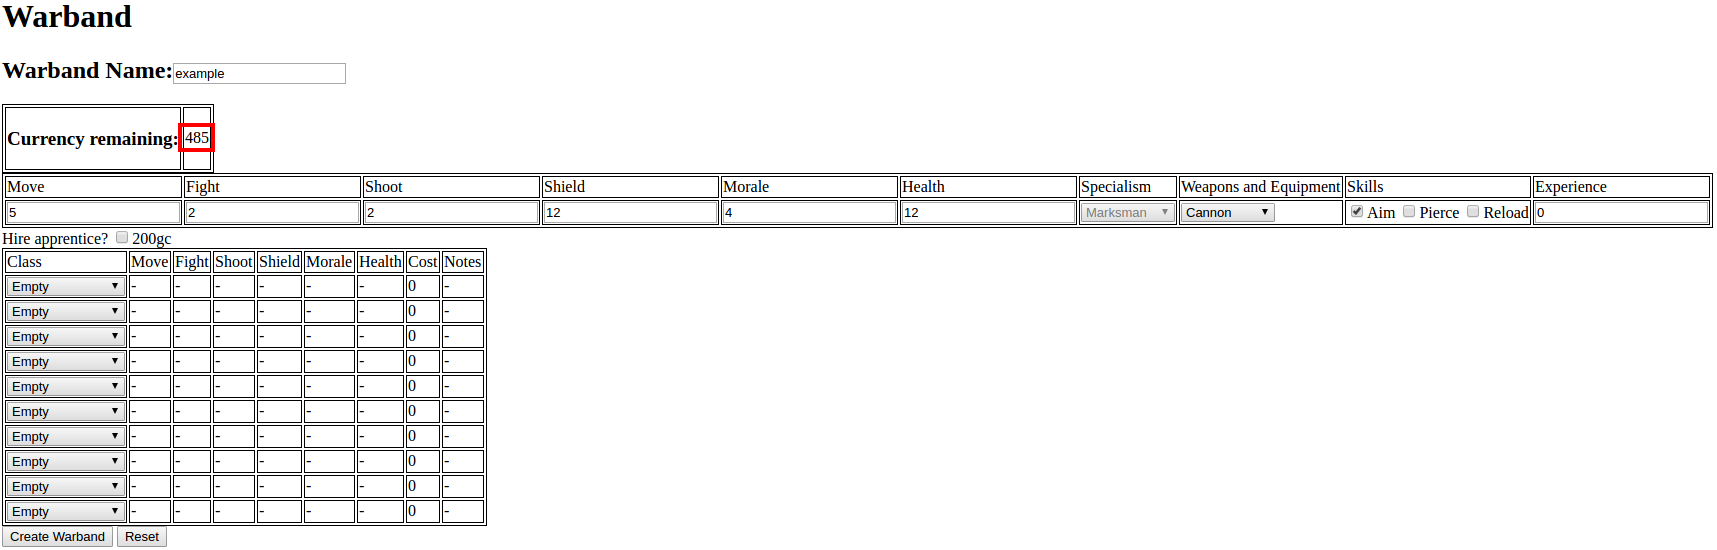
\includegraphics[width=1\textwidth]{img/example00}
 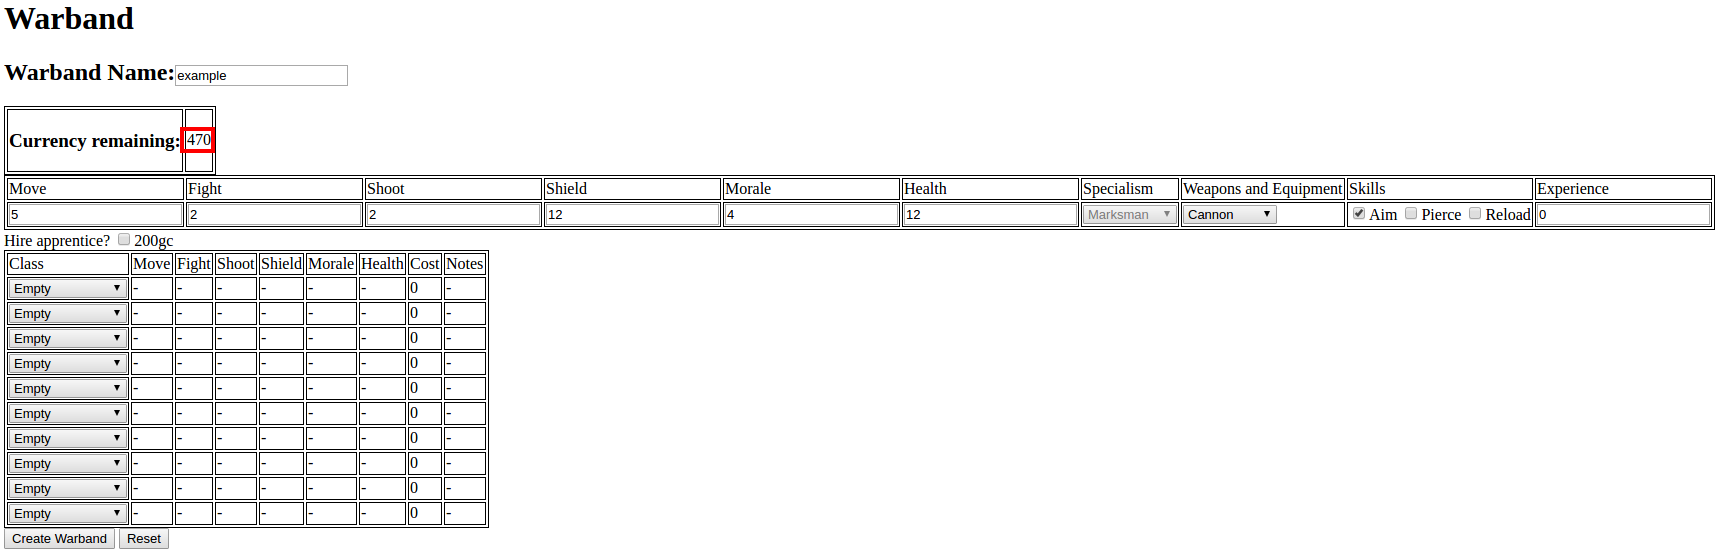
\includegraphics[width=1\textwidth]{img/example01}
 \end{minipage}
 
 \item It is not possible to hire an Ensign after creating the Warband.
 \item Squad members are treated like slaves, i.e. it is possible to sell them for the original amount of credits that they were ``hired'' with. This needs to change according to the game rules.
 \item The rules for increasing the Captain's and Ensign's skills is completely off - it is unlimited and completely uncorrelated to the experience points.
 \item There is also no limit regarding the amount of experience points that can be added with a single edit.
 \item The Captain and Ensign maximum values of skills (Annex) are not taken into consideration.
 \item Captain is not able to have \textbf{two} weapons.
 \item Neither Captain nor Ensign can obtain extra equipment.
 \item When attempting to make an illegal Warband nothing happens - not even the generic error message returned previously.
 \item Impossible to add number of credits.
\end{enumerate}

The past two lists were obtained exclusively from using the current web application, and valuable information was extracted from this method. The focus of the report will return to this in section~\ref{sec:sols} for proposed solutions for the mentioned problems. These are, obviously, intimately linked to the problems found in the current source code. Thus it is also important to review the actual files that have generated the web application. An overview of the \texttt{python} files that are used for going back and forth between \texttt{html} files, as well as the actual \texttt{html} files is done. 

\subsection{\texttt{.py} and \texttt{.html} Files}

The following lists some problems found with the given \texttt{python} script that is used to navigate inside the web application dealing with checking (or attempting to check) the validity of new or edited Warbands as well as the \texttt{html} files.  

\begin{enumerate}
 \item An important thing that must be considered is that this application does not install (or even check) for the dependencies it has (\texttt{Flask} is not among \texttt{python}'s built-in modules).
 \item The application assumes that \texttt{python} is installed, while this might not be the case. 
 \item The use of \texttt{flask} framework requires an installation in many machines.
 \item \texttt{framework.py} uses cryptic names like \texttt{wizard} to refer to the Captain, or \texttt{apprentice} to refer to the Ensign.
 \item The \texttt{framework.py} file is not written for humans: Horrible style and formatting and almost no comments are used in the code.\\
 \begin{minipage}[t]{\linewidth}
 \centering
 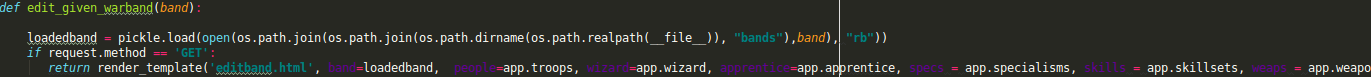
\includegraphics[width=1\textwidth]{img/formatting}
 Careless formatting.
 \end{minipage}
 
 \item There is no \texttt{try/except} methods for actions that could incur in errors. For example, opening files in \texttt{framework.py}.
 \item The validate functions (check that there's a positive number of credits, number of squad members, etc.) need to be written. 
 %\item Using \texttt{createdband} variable name everywhere in the \texttt{new\_band} function relates to problem 3.1.10.%\\
 %\begin{minipage}[t]{\linewidth}
 %\centering
 %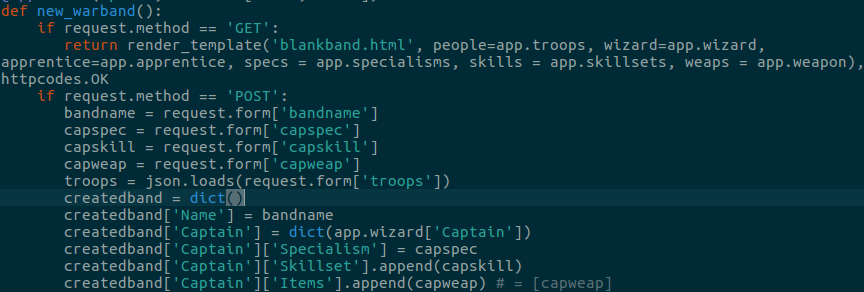
\includegraphics[width=1\textwidth]{img/new_warband}
 %Problem when creating new warband.
 %\end{minipage}
 
 \item \texttt{framework.py}'s \texttt{sumband} function works incorrectly when an Ensign is included - it adds the Captain's weapons twice instead of summing the Captain's and the Ensign's weapons. (Related to problem 3.1.10).\\
 \begin{minipage}[t]{\linewidth}
 \centering
 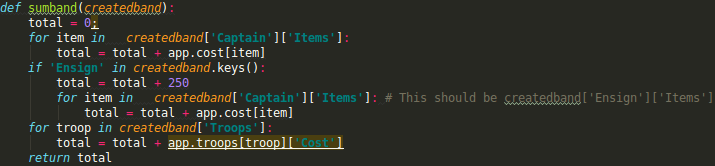
\includegraphics[width=1\textwidth]{img/sumband}
 \texttt{sumband} error.
 \end{minipage}
 
 \item Use augmented assignment in \texttt{sumband} function.
 \item \texttt{bandlist.html}, \texttt{blankband.html}, and \texttt{editband.html} show no route to go to \texttt{index.html} - this should be supported.
 \item \texttt{blankband.html} and \texttt{editband.html} have strange formatting decisions.
 \item \texttt{blankband.html} and \texttt{editband.html} mistakes the name of the Ensign with ``Apprentice''. This is related to problem 3.1.6.
 \item \texttt{blankband.html}'s \texttt{hireEng()} function uses a hardcoded (mistaken) value for the Ensign's hiring price. This is related to problem 3.1.7.\\
 \begin{minipage}[t]{\linewidth}
 \centering
 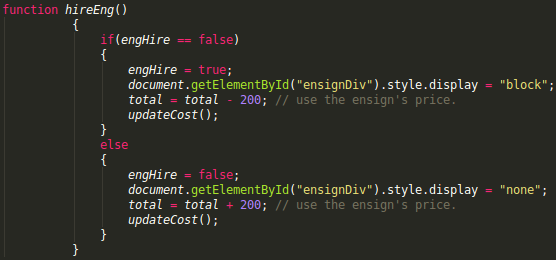
\includegraphics[width=1\textwidth]{img/hireEng}
 Hardcoded values in \texttt{hireEng()} function.
 \end{minipage}
 
 \item \texttt{editband.html} and \texttt{blankband} have several formatting errors - again, not designed for humans.
\end{enumerate}

These are the problems found in the web application source files. Nevertheless, they are probably just scratching the surface, and when the process of fixing them starts, considerably more problems will be discovered. As it was mentioned in the introduction section, it is important to take into account the level of experience at hand. Having no knowledge of \texttt{Flask}, \texttt{JavaScript} or \texttt{html} a learning curve behaviour will need to be included in time and effort estimations. 

This means that two factors will increase the uncertainty of the project planning. Both are directly related to a lack of experience in the programming languages that are used in the current code. The first factor is that the errors identified in the current report constitute only a fraction of the entirety of errors that actually exist in it. This will need to be included in the project planning (Gantt chart) in the form of an increase in the time needed to fix all problems in the code. This will be done through a combination of estimation and accountability of research/study time: tutorials of \texttt{Flask} and \texttt{html} (the main source of uncertainty at the moment) will make up around 8 to 10 work hours in the Gantt chart, and by considering that the number of problems found will be roughly double the number of problems that this report has found (only considering section 3.3). 


\section{Solution Proposals}
\label{sec:sols}

The problems identified in the previous section are, in general, not extensively complicated. Some of them require previous knowledge, and thus will require more time than others. A subset of these problems -- those related to the multiplayer implementation -- requires the most amount of effort. Similarly, becoming acquainted with \texttt{html} will require some effort at the beginning. Throughout the progress of the project, time is allocated for error handling and testing.  

The problems are classified as follows:

\begin{enumerate}
 \item Formatting problems. For close to 1200 lines of code (generally not the best metric for estimations, but this is solely for formatting), around 2 to 3 hours will be required with the help of an adequate IDE. This also includes fixing cryptic names, style, formatting and comments. This is imperative before starting any coding, and also important before delivering the end product (it has to be properly commented).
 \item Dependencies problems - implement methods that check the presence of \texttt{Flask} and other dependencies. In the end it should install the required modules such that the application can run smoothly. Around 1 to 2 hours to complete. This can be done among the final tasks - when all the necessary modules will be referenced to.
 \item Validate functions. This will be among the first few methods to go deep into the code, so a thorough understanding of it is necessary. Some effort has to be directed at familiarising with the \texttt{flask} framework. Around 3 to 5 hours.
 \item Update functions. This will deal with experience points conversion to skills in a legal manner, Captain and Ensign's extra weapons or equipment, addition of credits, removing squad members, and many more (including any problems that are found in the future). Around 5 to 6 hours. 
 \item \texttt{html} tutorial. Going through a basic \texttt{html} tutorial and writing methods to go from ``Edit'' or ``New'' Warband menus to ``Home''. Around 2 to 4 hours.
 \item \texttt{html} functions. Go through problems 3.3.11-13, and very likely find several more errors. Around 5 hours.
 \item Internal error message handling. This relates implementing \texttt{try/except} and \texttt{assert} methods to handle errors and help in unit testing. This is something that needs to be done throughout the coding process - around 2 to 4 hours.
 \item External error message handling. This relates to problem 3.1.3, and means identifying illegal squads and writing \texttt{html} error messages (with ways to return to ``Back'' or ``Home''. Without considering the time for writing the validate functions, around 1 to 2 hours to complete.
 \item Multiplayer 1. Web application security tutorial and implementation of login with player name and password (talk with client first). Only the Warband's owner can edit it, but everyone else can see it. Around 4 to 7 hours.
 \item Multiplayer 2. Implement the web application for multiplayer, adding player's name to the Warband's information. Around 4 to 7 hours hours.
 \item Testing. Repeat previous tasks to keep consistency with previous advancements. Around 1 to 2 hours.
\end{enumerate}

\section{Time/Effort Estimation Plan}

This section features a Gantt chart that uses the problems found on the code as well as the proposed solutions as a guideline. Said chart summarises the proposed solutions with the estimation of the effort and time that each of them will require. Several instances of error handling and testing are allocated in the Gantt chart. This is very important to produce a well rounded end product and intimately related to the fact that the chosen development model is the waterfall with subprojects (this will be further discused in the following section).

\newganttchartelement{voidbar}{
 voidbar/.style={draw=black, top color=black!25,bottom color=black!23}
}
\begin{ganttchart}[x unit=0.42cm, y unit title=0.7cm, y unit chart=0.5cm, vgrid, title label font=\footnotesize,canvas/.style={draw=black, dotted}]{1}{26}
        \gantttitle{Hours}{26}\\
        \gantttitlelist{0,5,10,15,20,25,30,35,40,45,50,55,60}{2} \\

        \ganttbar{Formatting}{1}{1}     \\ 
        \ganttbar{Validate}{2}{3}    \\
        \ganttbar{Testing}{4}{4} \\
        \ganttbar{\texttt{html} tutorial}{5}{6}              \\ 
        \ganttbar{\texttt{html} functions}{7}{8} \\
        \ganttbar{Internal EH}{9}{9} \\
        \ganttbar{Update functions}{10}{12} \\
        \ganttbar{External EH}{13}{13}\\
        \ganttbar{Testing}{14}{14} \\
        \ganttbar{Multiplayer 1}{15}{17} \\
        \ganttbar{Multiplayer 2}{18}{19} \\
        \ganttbar{Internal EH}{20}{20} \\
        \ganttbar{Testing}{21}{22} \\
        \ganttbar{External EH}{23}{23} \\
        \ganttbar{Dependencies}{24}{24} \\
        \ganttbar{Testing}{25}{26}
\end{ganttchart}
    
\section{Risk Analysis and Management Strategy}

As it was mentioned before, the strategy that will be used for the development of this project will follow the waterfall with subprojects model. For this model, the software concept and the requirements analysis have been already covered and explained in section~\ref{sec:concept}. 

The architectural design of the web application has already been built and exists in the provided code, but has to be extended to multiplayer support. Before doing so, one full ``loop'' from architectural design to testing and back is performed. Afterwards, the multiplayer support is created and a full loop is done once more. A few instances of error handling are also used in order to catch errors through the code. 

\begin{figure}[ht]
 \centering
 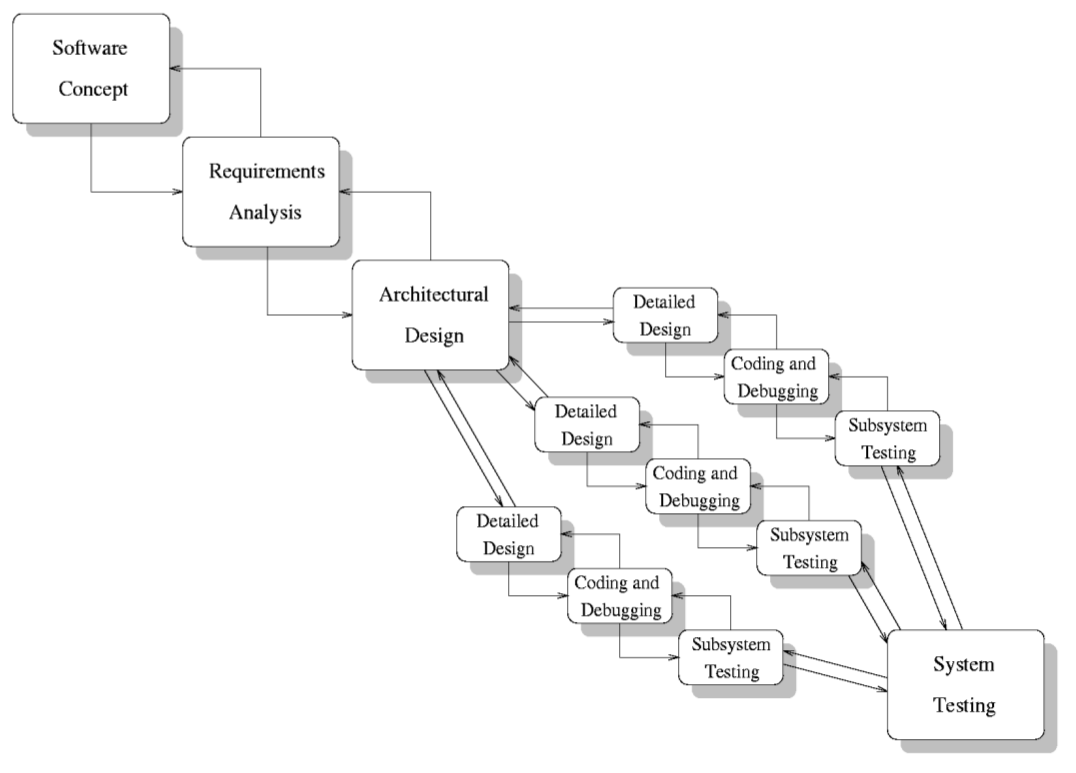
\includegraphics[width=0.8\textwidth]{img/waterfall_subp}
 \caption{Waterfall with subprojects}
\end{figure}

The processes that have been mentioned help with risk management. Throughout the improvement of the code it is necessary to check if the Warbands that are being generated are legal before and after dealing with the multiplayer platform. The Gantt chart attempts to account for this through systematically testing as well as Internal and external error handling. Another possible risk that is mitigated by the project planning is the possible dependencies that the application may need. 

The largest risk is, as has already been mentioned, the lack of experience in many aspects of the project's current build. This has been referenced several times and it is something that is being taken into consideration through the development of the project planning. This has been accounted into the necessary time for ``preparation'' for some of the tasks. 


\newpage

\section{Annex}

\subsection{Base stats}

Besides the stats shown in table~\ref{Atable:1}, both Captain and Ensign start with empty Skillset (that has to be filled when creating a squad), as well as an Associated Specialism, and no Items (one Weapon has to be added when creating a squad). All other stats are summarized in the following table.

\begin{table}[h]
\begin{center}
\begin{tabular}{|m{1.8cm}|c|c|c|c|c|c|c| m{2.1cm} |}
\hline
{\bf Squad Member} & {\bf Move} & {\bf Fight} & {\bf Shoot} & {\bf Shield} & {\bf Morale} & {\bf Health} & {\bf Cost} & {\bf Experience}\\
\hline
  Captain & 5 & 2 & 2 & 12 & 4 & 12 & 0 & 0\\
  \hline
  Ensign & 7 & 0 & -1 & 10 & 2 & 8 & 250 & 0\\
  \hline
  & & & & & & & & {\bf Notes} \\
  \hline
  Augment Gorilla & 8 & 3 & 0 & 10 & 2 & 8 & 20 & Animal, cannot carry treasure or items\\
  \hline
  Lackey & 6 & 2 & 0 & 10 & -1 & 10 & 20 & Melee Weapon\\
  \hline
  Security & 6 & 2 & 1 & 12 & 2 & 12 & 80 & Blaster, Blade\\
  \hline
  Engineer & 4 & 0 & 3 & 12 & 2 & 10 & 60 & Blaster, Repair Kit\\
  \hline
  Medic & 5 & 0 & 0 & 12 & 3 & 10 & 50 & Blade, Medkit\\
  \hline
  Commando & 8 & 4 & 0 & 10 & 4 & 12 & 100 & Stealth Suit, Blade, Needle Gun\\
  \hline
  Combat Droid & 3 & 2 & 4 & 14 & 0 & 14 & 150 & Mechanoid, Dual Blaster, Claws\\
\hline
\end{tabular}
\end{center}
\caption{Base stats for each squad member.}
\label{Atable:1}
\end{table}

\newpage

\subsection{Maximum Stats}

As the Captain and Ensign are able to increase their stats, it's important to state their maximum stats. In order to increase any of these stats by \textbf{1} point, the corresponding squad member (Captain or Ensign) will loose \textbf{10} EXPERIENCE points. In one edit no stat can be increased by \textbf{more than 1} point.

\begin{table}[!ht]
\begin{center}
\begin{tabular}{|c|c|c|c|c|c|c|c|}
\hline
{\bf Squad Member} & {\bf Move} & {\bf Fight} & {\bf Shoot} & {\bf Shield} & {\bf Morale} & {\bf Health}\\
\hline
  Captain & 5 (+0) & 2 (+8) & 2 (+8) & 12 (+0) & 4 (+8) & 12 (+8)\\
  \hline
  Ensign & 7 (+0) & 0 (+6) & -1 (+6) & 10 (+0) & 2 (+4) & 8 (+8)\\
\hline
\end{tabular}
\end{center}
\caption{Maximum stats for Captain and Ensign.}
\label{simple_table}
\end{table}



%\begin{thebibliography}{100}

%\bibitem{ref:lam} L.Lamport. {\em 1986 Latex User's Guide
%and Reference Manual.} Addison Wesley. pp242.

%\bibitem{ref:bloggs} F.Bloggs. {\em 1993 Latex Users do it
%in Environments} Int. Journal of Silly Findings. pp 23-29.

%\end{thebibliography}


\end{document}

